\section{Background}
Many of todays smart phones are running Android as their operating system, and  data claims it dominates the market with an 87.6\% share in the second quarter of 2016\cite{idc}. Making it essenstial for future mobile forensic work, for gathering information in an investigation.

When an investigation occurs, there are several approaches to data acquisistion: (1) Manual acquisition, (2) Logical acquisition, (3) Physical acquisition, (4) Brute force acquisition. The field of interest for this paper is physical acquisition of the primary storage; it focuses primarly on creating a bit-by-bit copy of the random access memory (RAM). Due to RAM being volatile, it is often the target of stealthy illegal activites to avoid leaving data. If data was stored in the flash drive, it would still be resident until OS tries to overwrite the same physical area and garbage collector is initiated. The point being that data residing on a secondary storage device, will be living longer and probably be logged more extensively.

The Android OS is in short words a Linux-based OS, where most OS tasks are performed by open source C libraries, and Java is used for the development of Android applications. These applications are compiled to bytecode for the Java virtual machine (JVM), which is then translated for a second virtual machine which executes them. Depending on which version of Android a smart phone is running, different virtual machines are used for execution.
For Android versions 4.4 and prior, Dalvik was used. It was replaced by ART in 4.5, and is still the de-facto standard.

Why does this matter? The virtual machines that are used are suppose to run Java applications, and have therefore gained several features of the Java programming language. One of these features are the memory management module, which has a built-in garbage collector(GC). It lets the user create objects without worrying about memory allocation and deallocation. Reducing the need for boilerplate code, and problems with memory leaks and such, which often are languages like C and C++ are subject to. 

The GC have the job of cleaning RAM, therefore removing potential information to be gathered. It is therefore of severe importance, that data residing in memory gets gathered before the device eventually power offs, or the garbage collector initializes.

Both ART and Dalvik use by default a method called "concurrent mark and sweep" for their GC\cite{ARTGC,DALVIKGC}. It works by traversing the heap for objects that are "reachable" or used by applications, those who are not will be regarded as free space again. Making space for potential new data to be stored within it. A figure of the process, can be seen at figure \ref{fig:mas}. Generally the heap is a region of the memory that is regarded as free memory for any process to use, however in Java it is used to store all objects created. Therefore the GC may potentially remove one of the better sources for information, the objects. The good news are that once data is freed, no overwriting is enforced; in other words, data is not overwritten until another object takes its place\cite{DALVIKGC}; in addition to each application running its own garbage collector and private heap, making the RAM data resident for possibly long periods of time.

\begin{figure}[h]
  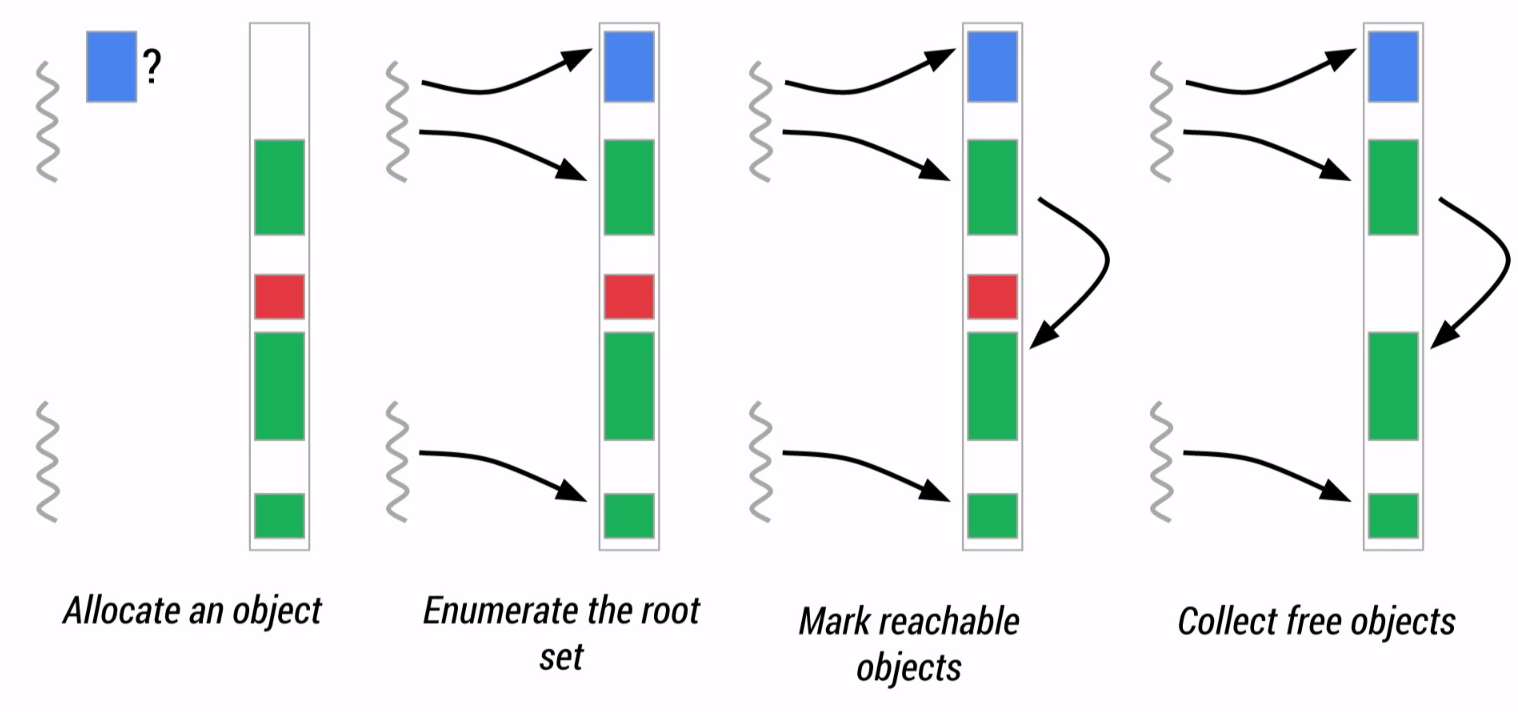
\includegraphics[width=0.5 \textwidth]{gc}
  \caption{Mark and Sweep\cite{ARTGC}}
  \label{fig:mas}
\end{figure}

Because all objects created in the heap, there may be a potential trace of information of an application. Through the use of several popular online communication applications, the amount of data that can be collected through a memory dump will be explored; despite knowing that the GC might start, or extra security measures might prevent us to do so.